\documentclass[11pt]{article}
\usepackage{graphicx}

\title{\textbf{Chisualizer Quick Start \& Reference}}
\author{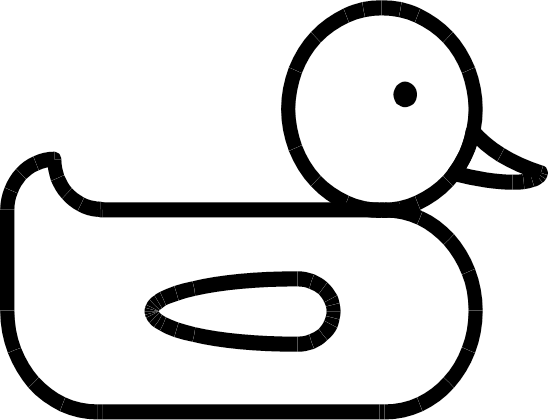
\includegraphics[scale=0.025]{bigduck} Ducky}
\date{24 Nov 2014}
\begin{document}

\maketitle


\section{Prerequisites}
The following software needs to be installed:
\begin{itemize}
  \item Python 2.7 (https://www.python.org/download/releases/2.7/)
  \item wxPython (http://wxpython.org/download.php)
  \item pyCairo (http://cairographics.org/pycairo/)
\end{itemize}

On a Debian or Ubuntu Linux machine, this command should install all the prereqs:
\begin{verbatim}
sudo apt-get python-wxgtk2.8 python-cairo
\end{verbatim}

On a Windows machine, you should be able to download the prereqs from the relevant sites. Note that the examples are reliant on Make and g++, which are not available standard on Windows machines.

\section{Known Issues}
\begin{itemize}
  \item Bundle subelements, normally accessed in Chisel through a dot (.), require an underscore (\_) in Chisualizer. So gcd.io.in.ready becomes gcd.io\_in\_ready - this is because of an issue with Chisel's name resolution system and requires an upstream fix.
\end{itemize}

\section{Quick Start Example: GCD}
\subsection{Building}
Clone the Chisualizer repository to your location of choice.
\begin{verbatim}
git clone https://github.com/ducky64/chisualizer.git
\end{verbatim}

Go into the GCD example directory, and build the GCD emulator. SBT will automatically pull Chisel from the latest version released. Or something like that.
\begin{verbatim}
cd chisualizer/tests/gcd
make
\end{verbatim}

\subsection{Running}
Once it's built, run the GCD example.
\begin{verbatim}
make run
\end{verbatim}

Note that the above is actually shorthand for the actual command to run the Chisualizer:
\begin{verbatim}
python ../../src/main.py  --emulator emulator/emulator --visualizer_desc gcd.yaml
pkill emulator
\end{verbatim}

(the pkill is necessary because of a bug where the spawned emulator subprocess does not stop when Chisualizer is terminated, and instead proceeds to eat up all your CPU)

You can navigate around the visualization using the mousewheel to zoom in and out. The circuit can be stepped forward and backwards in time using the arrow keys. Additional commands are listed at the bottom of the window.

You can right-click elements to bring up a context menu to perform actions, like changing circuit state. Double-clicking usually is shorthand for running the topmost element in the menu.

Try running the GCD of two numbers (say, 1337 and 42) by changing the state of the input operands and valid signal, then stepping until the calculation completes. Note that you can only change saved state (register values) - the circuit automatically updates (propagates values from registers) after each modification.

\section{A More Complex Example: DREAMER 3-stage}
Unlike GCD, DREAMER (a NoC manycore processor) code isn't publicly available. I'm not sure if the emulator builds easily either, so this will also be a tutorial of how to run Chisualizer with a dummy emulator. Dummy mode is where there is no actual backing circuit - every request for a node returns a width of 32 bits, a depth of 16 elements, and a value of zero. Try running the DREAMER visualizer:
From the Chisualizer repository base directory, run:
\begin{verbatim}
cd chisualizer/tests/fix-tile
./chisualizer-run-dummy.sh
\end{verbatim}

This shows a more realistic design with some notable features:
\begin{itemize}
  \item "Symbols" can be created using Unicode characters - like the directional arrows on the ready/valid
  \item You can have multiple windows showing different visualizations. All these are linked - so modifying state or stepping cycles on one will update all the others.
  \item In "multi3stage", if you right click anywhere, you can choose different views. The default is the "router" overview view, but you can also switch to the "full" detailed view.
  \item In "full3stage", you can see memory element highlighting in the regfile. The element being referred to by io\_reads\_*.adr is being highlighted with a green box.
  \item The mechanisms for these will be described in the Visualizer Descriptor Language Reference below.
\end{itemize}

\section{Visualizer Descriptor Language Reference}
Visualizer descriptors are how you tell Chisualizer how to render your circuit. They're written in a domain-specific language on top of YAML (of which JSON is a subset). You can see the examples ( \texttt{gcd.yaml} and \texttt{fix3stage.yaml}) as some examples.

The main concept is that visualizers (the visual representation of a node, module, or general circuit thing) are composable and semi-automatically placed and sized. Composable means you can put visualizers inside (some) visualizers, and semi-automatically placed and sized means that you only specify relative placement and the system will automatically determine the actual raw coordinates and required sizing. This is because working with raw coordinates, while powerful, is time-consuming and not amenable to change.

At the top level is a mapping (or dict, if you prefer) of:
\begin{itemize}
  \item \texttt{lib}: \texttt{mapping}(reference name$\rightarrow$\texttt{Visualizer}) \\
  \texttt{lib} specifies a library of visualizers that may be referenced later.

  \item \texttt{display}: \texttt{mapping}(title$\rightarrow$\texttt{Visualizer}) \\
  \texttt{display} specifies the \texttt{Visualizers} to render, one per window. The typical pattern for this is to specify references to the \texttt{Visualizers} described in \texttt{lib}.
  
  \item \texttt{temporal}: \texttt{mapping}(title$\rightarrow$\texttt{Visualizer}) \\
  \texttt{temporal} specifies the \texttt{Visualizers} to render as a temporal overview, one per window. Temporal overview is where the \texttt{Visualizer} is stacked in vertically in time. The typical use case is to describe a \texttt{Visualizer} that gives a good at-a-glance overview at a particular point in time.
\end{itemize}

\subsection{Basic Visualizers}
You're probably now wondering, "what's a \texttt{Visualizer}"? \texttt{Visualizers} are tagged mappings like such:
\begin{verbatim}
!TextBox {path: .state, template: gcd_state_map}
\end{verbatim}
The \texttt{!TextBox} is the tag (it's a \texttt{TextBox} object), and the mapping describes its attributes. Each attribute can either be dynamic (can change based on data value) or static (can't change), and has an associated data type. More on data types later.

A complete listing of Visualizers follows:
\begin{itemize}
  \item Common attributes to all Visualizers \\
  Only path, modifiers, and template are important, the rest control visual properties and have sensible defaults.
  \begin{itemize}
    \item \texttt{path} (\texttt{String}, static): The path component for this visualizer, joined to its parent's \texttt{path}. Use \texttt{.\_\_up\_\_} to go one level up from the parent (to the previous dot).
    \item \texttt{modifiers} (\texttt{list[Modifiers]}, static): A list of \texttt{Modifiers} (objects that can modify either this \texttt{Visualizer}'s or a child's attributes based on circuit data). Current only applicable to \texttt{MemoryArrays}.
    \item \texttt{template} (\texttt{String}/ref, static): Inherit attributes from a \texttt{Template} object.
    
    \item \texttt{frame\_style} (\texttt{String} [\texttt{none}, \texttt{frame}], static): Whether this Visualizer should be rendered with a graphical frame (margin) around it.
    \item \texttt{frame\_margin} (\texttt{Int}, static): Size of the frame.
    \item \texttt{border\_style} (\texttt{String} [\texttt{none}, \texttt{border}], dynamic): Whether this \texttt{Visualizer} should be rendered with a graphical box around it in the center of the frame margin. Obviously, \texttt{frame\_style} must be \texttt{frame}.
    \item \texttt{border\_size} (\texttt{Int}, static): Size of the border.
    \item \texttt{border\_color} (\texttt{String/color}, static): Color of the border.
    \item \texttt{label} (\texttt{String}, static): Label text to put in the border. If left empty, this will display a cleaned version of \texttt{path}.
    \item \texttt{label\_size} (\texttt{Int}, static): Font size for the label.
    \item \texttt{label\_font} (\texttt{String}/font, static): Font for the label.
    \item \texttt{label\_color} (\texttt{String}/color, static): Color for the label.
  \end{itemize}
  \item \texttt{TextBox} \\
  \texttt{TextBox} is exactly what it says on the tin, a box with text. \\
  Only \texttt{text} is important, the rest control visual properties and have sensible defaults.
  \begin{itemize}
    \item \texttt{text} (\texttt{String}, dynamic): Text to display.
    \item \texttt{text\_size} (\texttt{Int}, static): Font size for the text.
    \item \texttt{text\_font} (\texttt{String/font}, static): Font for the text.
    \item \texttt{text\_color} (\texttt{String/color}, static): Color for the text.
  \end{itemize}
  \item \texttt{LineGrid} \\
  \texttt{LineGrid} is a container of \texttt{Visualizers}, putting them next to either other in a line that goes either horizontally (\texttt{dir=row}) or vertically (\texttt{dir=col}). \\
  TODO: There will be a picture here to help describe this concept sometime.
  \begin{itemize}
    \item \texttt{dir} (\texttt{String} [\texttt{row}, \texttt{col}], static): Whether cells are arranged left to right (\texttt{row}) or top to bottom (\texttt{col}).
    \item \texttt{cells} (\texttt{list[Visualizer]}, static): Children \texttt{Visualizers} to arrange in a line.
  \end{itemize}  
  \item \texttt{MultiView} \\
  \texttt{MultiView} allows the user to interactively switch between different \texttt{Visualizer}s. Useful for being able to change on demand between overview and detail views.
  \begin{itemize}
    \item \texttt{views} (\texttt{mapping[String$\rightarrow$Visualizer]}, static): Name and \texttt{Visualizer} associated with each different view.
  \end{itemize}
  \item \texttt{MemoryArray} \\
  \texttt{MemoryArray} is an grid of child \texttt{Visualizer}s, where each one is associated with a cell in a Chisel \texttt{Mem}. The grid will be automatically sized based on the memory depth and the specified number of rows and columns.
  \begin{itemize}
    \item \texttt{dir} (\texttt{String} [\texttt{row}, \texttt{col}], static): Direction of element index increment.
    \item \texttt{rows} (\texttt{Int}, static): Number of rows to display.
    \item \texttt{cols} (\texttt{Int}, static): Number of rows to display.
    \item \texttt{offset} (\texttt{Int}, dynamic): Offset (in element index) of the array. TODO: Well, it's supposed to be dynamic, anyways.
    \item \texttt{offset\_anchor} (\texttt{Int}, static): Percentage anchor of the offset. 0 would mean the offset is anchored at the beginning of the visible array, while 50 would mean the center. \\ TODO: This may be changed to a float between 0 and 1.
    \item \texttt{cell} (\texttt{Visualizer}, static): Visualizer to instantiate for each memory element visible.
  \end{itemize}
\end{itemize}

\subsection {"Syntactic Sugar" Visualizers}
\begin{itemize}
  \item \texttt{MultiLineGrid} \\
  \texttt{MultiLineGrid} is a convenient way to specify \texttt{LineGrid}s within \texttt{LineGrid}s. This extends the \texttt{LineGrid} syntax by allowing nested \texttt{list}s inside \texttt{cells}, which means to instantiate an \texttt{LineGrid} with \texttt{dir} opposite its parent.
  \item \texttt{Ref} \\
  \texttt{Ref} is a way to reference another \texttt{lib}-level \texttt{Visualizer} by reference name.
  \begin{itemize}
    \item \texttt{ref} (\texttt{String}, static): \texttt{lib}-level reference name of the \texttt{Visualizer} to reference.
  \end{itemize}
\end{itemize}

\subsection {Data Types}
The Chisualizer-specific data types referenced above (\texttt{String} and \texttt{Int}) are described in more detail here. Note the capitalization, to distinguish them from generic or YAML data types (like \texttt{string}s and \texttt{list}s).
\subsubsection {String}
This data type resolves to a \texttt{string}. In addition to regular YAML \texttt{string}s, the following objects are available for dynamic, data-dependent strings:
\begin{itemize}
  \item Common Attributes
  \begin{itemize}
    \item \texttt{path} (\texttt{String}, static): Path from the parent Visualizer, same semantics as \texttt{path} in \texttt{Visualizer}. Highly recommended to be left blank (to be consistent with the parent \texttt{Visualizer}).
  \end{itemize}    
  \item \texttt{NumericalString} \\
  The string representation of a number. Highly customizable.
  \begin{itemize}
    \item \texttt{prefix} (\texttt{String}, static): String prefix.
    \item \texttt{radix} (\texttt{Int}, static): Radix of the conversion.
    \item \texttt{charmap} (\texttt{String}, static): Character map for the conversion, typically \texttt{0123456789abcdef}.
  \end{itemize}
  \item \texttt{DictString} \\
  Mappings of specific numbers to strings.
  \begin{itemize}
    \item \texttt{mapping} (\texttt{mapping[Int$\rightarrow$String]}, static): \texttt{String} to return for the input (key) data value. \texttt{default} is also a valid key.
  \end{itemize}
\end{itemize}
  
These special semantic meanings are available (denoted in the references above as \texttt{String}/color, for example):
\begin{itemize}
  \item \texttt{String}/ref \\
  A reference (by name) to a \texttt{lib}-level \texttt{Visualizer}.
  \item \texttt{String}/font \\
  A font name. If this is invalid, the system will generally select some default font to use.
  \item \texttt{String}/color \\
  A color. Currently, valid values are: \texttt{black, red, yellow, green, cyan, blue, pink, white, grey}. Use of \texttt{black} and \texttt{white} are discouraged, as they are background colors for the default \texttt{Light} and \texttt{Dark} themes. The exact RGB values of the color may differ by selected theme.
\end{itemize}
  
\subsubsection {Int}
This data type resolves to an integer. Currently, only YAML integers (static) are available. \\
TODO: add dynamic integer objects.

\subsection {Templates}
\texttt{Templates} are a \texttt{mapping} of attributes to values which are inherited by any object inheriting it. These \texttt{template} objects are available:
\begin{itemize}
  \item \texttt{Template} \\
  A \texttt{Template}, nothing special to see here.
  \item \texttt{DictTemplate} \\
  This is a simple way to construct a \texttt{Template} with attributes of \texttt{DictString} objects grouped by a common data key.
  \begin{itemize}
    \item \texttt{mapping} (\texttt{mapping[Int$\rightarrow$mapping[attribute name$\rightarrow$String]]}, static): the mapping from the data value to the attribute to the \texttt{String} value. Seriously, do yourself a favor and try to learn by example instead of figuring out the theoretics. See \texttt{gcd\_state\_map} inside \texttt{gcd.yaml}.
  \end{itemize}
\end{itemize}

That's it.
\end{document}
